\documentclass[a4paper, 12pt]{ppgeb}

% |--- Títulos, autor, banca ---|----------------------{{{
% Autor:
% Substituta  as informações nos comandos a seguir, até a linha começando
% com \membrobancaexterno.
% Em \title: título na forma principal, como aparecerá em algumas páginas
% Em \tituloficha: título como aparecerá na ficha catalográfica; idêntico
% ao anterior, mas com possíveis quebras manuais de linha (usar \\ quando
% necessário, para ajustar as mudanças de linha na ficha catalográfica).
% Em   \titulocapaA,   \titulocapaB,   \titulocapaC:  título para a capa,
% dividido em no  máximo 3  linhas (coloque uma  linha em  cada  comando,
% dividindo como ficar melhor esteticamente).
% Remova  o  símbolo  de  comentário  (%)  de  \coorientador,  se  houver
% coorientador.
%  Em  \publicacao{011A/2019}:  o  número  final  será   fornecido   pela

\title{Modelo para dissertações do \\Programa de Pós-Graduação em Engenharia Biomédica}
\tituloficha{Modelo para dissertações do Programa de Pós-Graduação em Engenharia Biomédica\\\phantom{}[Distrito Federal], 2019.} 
\titulocapaA{Modelo para dissertações do}
\titulocapaB{Programa de Pós-Graduação em Engenharia Biomédica}
\titulocapaC{}
\titulofichadois{Modelo para dissertações no Programa de Pós-Graduação em Engenharia Biomédica}
\author{Claude Shannon}
\nomeinvertido{Shannon, Claude}
\orientador{Frank Lauren Hitchcock}
%\coorientador{Nome do Coorientador}
\publicacao{011A/2019}
\data{julho de 2019}
\ano{2019}
\areaum{Radioterapia} % Preencher com termos escolhidos para identificar a área
\areadois{Radioterapia de Intensidade Modulada (IMRT)}
\areatres{Dosimetria}
\areaquatro{Controle de qualidade}
\endereco{email-do-candidato@unb.br}
\cep{CEP xxxxx-xxx}

\membrobancainterno{Dr. Membro Interno}
\membrobancaexterno{Dr. Membro Externo}
%---}}}

% |--- Bibliotecas utilizadas ---|----------------------{{{
\usepackage[margin=1in]{geometry}
\usepackage{setspace}
\usepackage{multirow}
\usepackage{booktabs}
 \usepackage[brazil]{babel}
\usepackage{xfrac}
\usepackage{hyperref}
\hypersetup{
colorlinks = true,
linkcolor = black,
anchorcolor = blue,
citecolor = blue,
filecolor = blue,
urlcolor = blue
}
\usepackage{rotating}
\usepackage[margin=0.40in,font=small,labelfont=bf,labelsep=period]{caption}
%---}}}

% |- Formato de referências (use apenas uma das 2 linhas seguintes; comente a outra) -|-{{{
\newcommand{\formatobibliografia}{numero}
%\newcommand{\formatobibliografia}{autorano}

\ifthenelse{\equal{\formatobibliografia}{numero}}{
\bibliographystyle{plain}
}
{}

\ifthenelse{\equal{\formatobibliografia}{autorano}}{
\usepackage{apalike}
\bibliographystyle{apalike}
}
{}
%---}}}

% |--- Espaçamento, configuração de título de seções ---|----------------------{{{
\onehalfspacing

\makeatletter
\renewcommand{\section}{\@startsection
{section}
{1}
{0mm}
{-\baselineskip}
{0.5\baselineskip}
{\large\bfseries\scshape}}
\makeatother

\makeatletter
\renewcommand{\subsection}{\@startsection
{subsection}
{2}
{0mm}
{-\baselineskip}
{0.5\baselineskip}
{\bf\sffamily}}
\makeatother

\makeatletter
\renewcommand{\subsubsection}{\@startsection
{subsubsection}
{3}
{0mm}
{-\baselineskip}
{0.5\baselineskip}
{\bf\sffamily}}
\makeatother

\setlength{\parindent}{20pt}
\setlength{\parskip}{06pt}
\newcommand{\spaceinitialsname}{0.4mm}
\newcommand{\porcento}{\scalebox{0.5}{~}\scalebox{0.9}{\%}}
\newcommand{\scanner}{\emph{scanner}}
\newcommand{\scanners}{\emph{scanners}}
\newcommand{\cmcubico}{${\textrm{cm}^{\scalebox{0.7}{3} }}$}
\setcounter{secnumdepth}{3}
%\setcounter{tocdepth}{3}
%---}}}

% |--- Comandos especiais ---|----------------------{{{
\newcommand{\cmquad}{${\textrm{cm}^{\scalebox{0.7}{2}} }$}
\newcommand{\mmquad}{${\textrm{mm}^{\scalebox{0.7}{2}} }$}
\newcommand{\gcmquad}{${\textrm{g}}/{\textrm{cm}^{\scalebox{0.7}{2}} }$}
\newcommand{\subsecref}[1]{Seção~\ref{#1}}
\newcommand{\figref}[1]{Figura~\ref{#1}}
\newcommand{\etal}{\emph{et~al.}}
\newcommand{\Jawsonly}{{\emph{Jaws-Only}} }
\newcommand{\jawsonly}{{\emph{jaws-only}} }
\newcommand{\software}{\emph{software}}
\newcommand{\percentagesignscale}{0.8}
\newcommand{\percent}{\scalebox{\percentagesignscale}{~\%}}
\newcommand{\subsubsubsection}[1]{\vspace{16pt}\noindent\textbf{#1}\\[12pt]}
%---}}}

% |--- Diretório(s) com figuras (se desejar, inclua subdiretórios) ---|-------------{{{
\graphicspath{{figuras/}}
%---}}}

% |--- Lista de palavras que não podem ser separadas em sílabas ---|------------------{{{
\hyphenation{development results Commissioning possibility Philadelphia Devic Calculations Calculation Language}
%---}}}

% |--- Texto principal ---|----------------------{{{
\begin{document}

\maketitle

% Se desejar uma epígrafe, remova o % do início das próximas linhas (até ==============)
%\clearpage
%\hspace{1mm}
%
%\vfill
%
%\hspace{1mm}
%
%\begin{center}
%\emph{Epígrafe} \\
%Autor da epígrafe
%\end{center}
%
%\hspace{1mm}
%
%\vfill
%
%\hspace{1mm} 
% ==============

% Se desejar uma dedicatória, remova o % do início das próximas linhas (até ==============)
%\clearpage
%\hspace{1mm}
%
%\vfill
%
%\begin{flushright}
%\begin{itshape}
%Texto da dedicatória.
%\end{itshape}
%\end{flushright}
% ==============

% Se desejar incluir agradecimentos, remova o % do início das próximas linhas (até ==============)
% \clearpage
%\noindent{\bfseries{\maiusc{\large Agradecimentos}} }
%
%\vspace{24pt} Agradecimentos
%
%\noindent 
%\clearpage
% ==============

\newgeometry{bottom=0.8in, top=0.9in, left=0.9in, right=0.9in}

\noindent{\bfseries{\maiusc{\large Resumo}} }
\acresetall % Manter essa linha!
\vspace{12pt}

Texto do resumo.

Esta seção deve sintetizar todo o trabalho, incluindo a definição do problema de pesquisa, os objetivos, a metodologia, resultados e conclusão. Note que não se trata, portanto, apenas de uma visão geral do trabalho, mas de um resumo de toda a dissertação.

O resumo pode ser dividido em parágrafos. A especificação de resumo em parágrafo único é comum a artigos de congressos e de periódicos, mas em dissertações e teses é permitida, dependendo do programa, a divisão em parágrafos.

\vspace{14pt}

\noindent{\textbf{Palavras-chave: }}inclua aqui as palavras-chave.
\acresetall % Manter essa linha!
\clearpage
\restoregeometry
% \chapter{Abstract}
\noindent{\bfseries{\maiusc{\large Abstract}} }
\acresetall % Manter essa linha!
\vspace{24pt}

Translation of the previous page into English.

Here you can also divide the text into paragraphs.

Do not overuse the passive voice. You should use the first person when describing what you developed yourself.

\vspace{14pt}

\noindent{\textbf{Keywords: }}include the keywords here.
\acresetall % Manter essa linha!

\indice

\begin{center}

{\bfseries{\maiusc{\large Lista de Nomenclaturas e Abreviações}} }%
\end{center}

\acrodef{3DCRT}[3DCRT]{Radioterapia Conformacional 3D, do inglês \emph{3D Conformal Radiotherapy}}
\acrodef{AAPM}[AAPM]{Associação Americana de Física na Medicina, do inglês \emph{American Association of Physics in Medicine}}
\acrodef{CQ}[CQ]{Controle de Qualidade}
\acrodef{SPT}[SPT]{Sistema de Planejamento de Tratamento}

\begin{acronym}
\acro{3DCRT}{Radioterapia Conformacional 3D, do inglês \emph{3D Conformal Radiotherapy}}
\acro{AAPM}{Associação Americana de Física na Medicina, do inglês \emph{American Association of Physics in Medicine}}
\acro{CQ}{Controle de Qualidade}
\acro{SPT}{Sistema de Planejamento de Tratamento}
\end{acronym}

\clearpage

\pagenumbering{arabic}

\acresetall % Manter essa linha!

\chapter{Introdução}

A introdução deve apresentar uma contextualização sobre o tema de pesquisa, culminando nas lacunas de pesquisa e na definição de uma proposta científica diante destas lacunas. Esclareça seus objetivos de pesquisa, deixando claras as hipóteses e perguntas científicas.

Se você deseja que o primeiro parágrafo de cada seção também tenha indentação, inclua no preâmbulo o comando \verb,\usepackage{indentfirst},.

Organize o texto em seções bem dimensionadas. Escreva de forma objetiva, usando conceitos claros e evitando comparações de caráter subjetivo. Evite frases muito longas.

A escolha dos títulos das seções cabe ao autor, mas é comum haver uma seção especificamente para os objetivos, frequentemente dividida em uma subseção \emph{objetivo geral} e uma subseção \emph{objetivos específicos}, conforme ilustrado a seguir. É comum que haja uma ou mais seções antes disso para contextualização, definição do problema científico, proposta de pesquisa.

\section{Observações Sobre Citações}

Cada afirmação no texto deve ser embasada na literatura científica, com um uma citação ao final da afirmação (não só ao final do parágrafo), ou em argumentos ou dados próprios.

No caso da citação de um texto da literatura, não copiar o texto; \textbf{mesmo com a indicação da referência, isso constitui plágio}. Cópias de texto podem ser usadas em casos específicos (por exemplo, na discussão de textos literários ou na apresentações de definições técnicas consagradas), mas isso exige que seja usado um formato específico de transcrição (texto indentado, em itálico, com indicação explícita de que se trata de texto de outro autor).

Ao citar outros trabalhos, dê preferência a artigos científicos, de periódicos fortes na área de pesquisa. Durante a definição do problema de pesquisa, é importante que sejam incluídas referências recentes (ainda que haja, também, referências mais antigas).

Você pode escolher um dos seguintes formatos para citação:
\begin{enumerate}[a)]
\item Citação pelo número da referência entre colchetes, conforme o exemplo a seguir~\cite{Kachuee2017}. Neste caso, os itens das lista de referências devem ser também numerados, com o número entre colchetes ao início de cada item. Os itens devem aparecer na lista em ordem alfabética do nome de família de cada autor. Nomes de instituições têm a ordem definida pelo nome inicial. Veja o exemplo no final deste modelo; cabe observar que é errada a ideia de que no caso de citações por número a lista de referências é sempre ordenada pela ordem de citação. Há ordenação pela ordem alfabética, como adotado pelo PPGEB e diversos outros programas, e por ordem de citação, como adotado por vários periódicos em que o número de citações é tipicamente bem menor.
\item Citação por autor e ano, conforme o exemplo a seguir~(Galahabi, 2017). Neste caso, o autor e ano aparecem entre parênteses, e a lista de referências não é numerada. Novamente os itens aparecem em ordem alfabética do nome da família de cada autor. Nomes de instituições têm a ordem definida pelo nome inicial. No caso de mais de um trabalho do mesmo autor no mesmo ano, inclua uma letra minúscula para diferenciá-los.
\end{enumerate}

Em LaTeX, para fazer uma citação use o comando \verb|\cite|, da seguinte forma. Após a informação a ser referenciada, coloque \verb|~\cite{chave}|, sendo \verb|chave| o identificador da referência a ser citada, conforme consta do arquivo \verb|referencias.bib|. Aqui, \verb|~| representa um espaço não-separável (não coloque caracter de espaço antes de \verb|~|). Veja os exemplos a seguir.

Uma primeira citação~\cite{Kachuee2017}. A lista de referências está em ordem alfabética, e neste exemplo o primeiro trabalho citado não é o primeiro da lista (não foi utilizada ordem de citação; coloque suas referências em ordem alfabética).

Segue um exemplo de citação~\cite{Gabriel2017}.

Outro exemplo~\cite{Ghahabi2017}.

Para citar vários trabalhos num mesmo ponto do texto, faça como neste exemplo~\cite{Kachuee2017,Gabriel2017,Ghahabi2017}.

Para símbolo de percentagem, utilize uma barra invertida antes (ou use o comando percent definido no preâmbulo). Exemplo: 37\percent.

\section{Observações Sobre o Uso de Siglas}

Quanto às siglas: sempre usar por extenso no primeiro uso, e colocar (no primeiro uso) a sigla entre parênteses. A partir do segundo uso, a sigla pode ser usada. Mas definições eventuais que tenham sido usadas no resumo não contam para o restante do texto, ou seja, se uma sigla foi definida e usada no resumo, ainda assim ela deve ser redefinida no primeiro uso após o resumo. Há comandos em LaTeX que facilitam esses procedimentos, conforme mostrado a seguir.

Exemplo de uso sigla. No serviço de radioterapia, o \ac{CQ} deve ser realizado segundo a norma XX/XX. O \ac{CQ} é normalmente acompanhado... 

A \ac{3DCRT} é normalmente usada... No Brasil, a \ac{3DCRT}...

Segundo a \ac{AAPM}, há duas formas... Essa orientação da \ac{AAPM} começou em...

O \ac{SPT} é um programa que permite o cálculo... Todo tratamento de radioterapia é baseado no \ac{SPT}.

\section{Objetivos}
\subsection{Objetivo Geral}

\subsection{Objetivos Específicos}

(Incluir as seções que se façam necessárias).

\chapter{Fundamentação Teórica}\label{chap:FT}

Este capítulo pode ter outro nome, e na verdade sugiro um nome mais específico (indique no título sobre o que trata a fundamentação em questão).

Inclua as seções que se façam necessárias.

\section{Observações Sobre Figuras}

Cada figura deve ser citada ao menos uma vez antes de aparecer no texto. As figuras devem ser numeradas no formato x.y, com x o número do capítulo e y o número da figura dentro do capítulo, e devem incluir uma legenda com o número e com um texto explicativo abaixo da figura em si. Como um exemplo, a Figura~\ref{fig:acelerador} ilustra um acelerador linear do Hospital Universitário de Brasília. Note que a citação foi com a palavra ``figura'' em letra maiúscula, como aparece na legenda. Note ainda que a legenda é em fonte menor do que o texto principal, e com margem reduzida em relação ao resto do texto.

\begin{figure}[h]
\centering
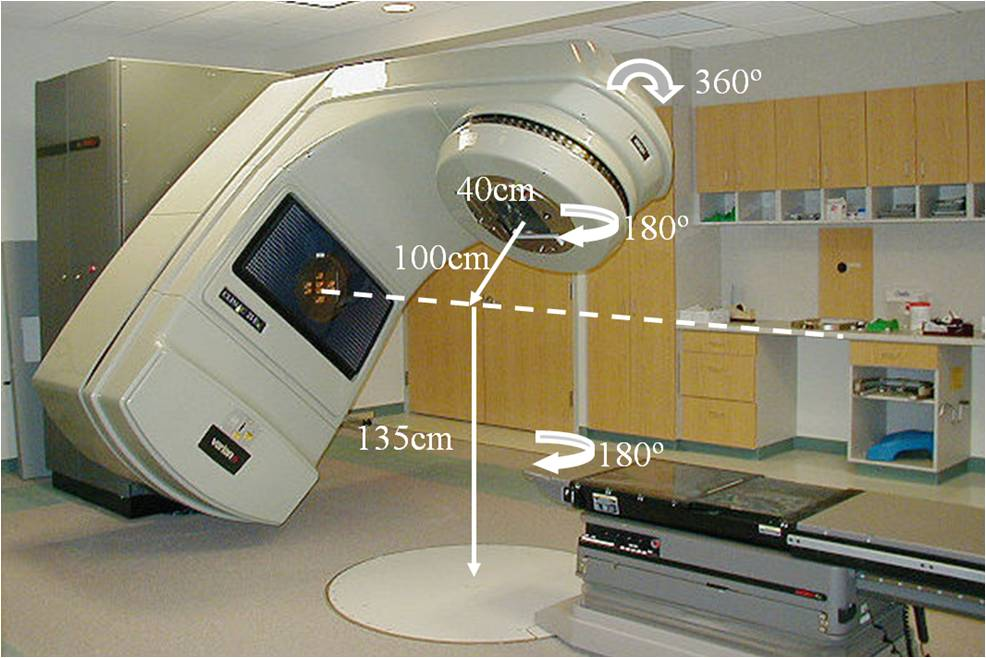
\includegraphics[width=100mm]{Acelerador2}
\caption[Exemplo de um acelerador linear utilizado no Hospital Universitário de Brasília.]{Exemplo de um acelerador linear utilizado no Hospital Universitário de Brasília. Os ângulos de 360${^{\textrm{o}} }$, 180${^{\textrm{o}} }$ e 180${^{\textrm{o}} }$ indicam os possíveis valores de rotação do acelerador e do \emph{gantry}. Os valores em centímetros indicam as dimensões do \emph{gantry} e as distâncias em relação à mesa e ao chão. Fonte:~\cite{Avelino2013}.}\label{fig:acelerador}
\end{figure}

Se você inserir figuras de outras fontes (livros, artigos, etc), deve incluir a fonte na legenda. Diga explicitamente ``Fonte: [X]'', sendo X a referência de onde foi tirada a figura. Ou use ``Adaptada de [X]'', caso a figura tenha sido modificada (por exemplo, traduzida). Não abuse, no entanto, da utilização de figuras de outras fontes. Dê preferência a trabalhos de sua autoria. Note que uma figura de outra fonte, mesmo com a devida citação, só poderia ser utilizada com autorização por escrito, para evitar processo por direitos autorais. Já o caso de inclusão de figuras de outras fontes sem a devida citação constitui plágio, sendo o autor do plágio sujeito à perda do título eventualmente obtido com a publicação e de outros direitos dela decorrentes.

\textbf{No caso de figuras de sua própria autoria, não indique isso na legenda. Não escreva, por exemplo, ``Fonte: o autor''}. Já se assume no texto que todo o material apresentado é produção do autor indicado, e os outros casos, que devem ser comparativamente poucos, é que devem ser explicitados.

\section{Observações Sobre Equações}

As equações são normalmente escritas de forma centralizada ao longo da direção horizontal, e com uma numeração à direita no caso das equações que são citadas. As equações que não são citadas posteriormente não precisam ser numeradas. Quando há numeração, ela aparece entre parênteses, e no formado x.y, com x o número do capítulo e y o número da equação dentro do capítulo.

Segue um exemplo de uma equação. Em um triângulo retângulo, a medida da hipotenusa é dada por
\begin{equation}\label{eq:hipotenusa}
a = \sqrt{b^2 + c^2},
\end{equation}
com ${b}$ e ${c}$ as medidas dos dois catetos.

Note em \eqref{eq:hipotenusa} que a equação faz parte do texto, no sentido de que ela não interrompe o fluxo da frase iniciada por ``Em um triângulo''. Não se deve, por exemplo, escrever ``a medida da hipotenusa é dada pela Equação 2.1'', e então colocar a equação abaixo como se fosse um objeto à parte do parágrafo (como acontece com as figuras e tabelas -- estas sim não se inserem no próprio texto, e são referenciadas como objetos independentes do parágrafo).

Por este motivo, as equações devem ser pontuadas conforme o texto normal. Elas devem ser seguidas, por exemplo, de ponto, vírgula, ou ponto-e-vírgula, conforme o fluxo do texto, a não ser que o texto imediatamente continue com a palavra ``e''.

Além disso, observe que todos os termos de uma equação que não foram previamente definidos devem ser definidos logo em seguida, como no caso de \eqref{eq:hipotenusa}. Os termos ${b}$ e ${c}$ foram definidos imediatamente após a equação. Nunca deve haver termos numa equação que não são explicitamente definidos no texto.

Segue um outro exemplo. A transformada discreta de Fourier de um sinal ${x}$ de comprimento ${N}$ é dada por
\begin{equation}
\hat{x}[k]=\sum_{n=0}^{N-1}x[n]\exp\left(-j\frac{2\pi nk}{N}\right),
\end{equation}
sendo ${j}$ a unidade imaginária e ${k}$ o índice de frequência considerado, com ${k\in\left\{0,1,\ldots,N\right\}}$.

\chapter{Materiais e Métodos}\label{chap:Metodologia}

Este capítulo pode ter outro nome, e na verdade sugiro um nome mais específico; indique no título sobre os tópicos metodológicos tratados. Pode ser usado mais de um capítulo para esses tópicos, se necessário.

Inclua as seções que se façam necessárias.

\section{Dicas para o capítulo}
Dicas importantes que devem ser contempladas neste capítulo, segundo~\cite{marconi.lakatos:2003}:
\begin{itemize}
\item Verificar se o capítulo responde as seguintes questões: Como? Com quê? Onde? Quanto?
\item A linguagem do projeto deve ser escrita com tempo verbal no futuro e da dissertação no passado.
\item É importante mencionar sobre: tipo de pesquisa (bibliográfica, descritiva, documental, experimental etc), dados (fonte de dados, forma de obtenção), população e amostra, tratamento e análise dos dados (descrição mais detalhada do método -- ou métodos -- que serão utilizados), limitações da pesquisa.
\end{itemize}

\section{Observações Sobre Quadros e Tabelas}

Quadros e tabelas são de uso semelhante às figuras, no que diz respeito à numeração, uso de legenda, e necessidade de citar ao menos uma vez antes da ocorrência. No entanto, no caso dos quadros e tabelas a legenda deve ser colocada acima, e não abaixo como nas figuras.

A Tabela~\ref{tab:exemplo} ilustra esse uso. Observe que a citação de uma tabela específica (pelo número) é com a palavra ``tabela'' em maiúscula, ao contrário da referência a tabelas em geral. Note que em uma tabela as bordas são horizontais (não use bordas verticais para separar colunas), e não são necessárias bordas para separar cada linha. Separe apenas as linhas do início, fim, e dos indicadores dos campos presentes, como no exemplo. Podem ser usadas bordas horizontais para separar regiões distintas de dados (seções de dados), se necessário.

\begin{table}[h]
\centering
\caption{Parâmetros utilizados na implementação do método de deteção de bordas proposto, em cada configuração considerada.}\label{tab:exemplo}
\begin{tabular}{ccllll}
\cline{1-5}
\multirow{2}{*}{Configuração} && \multicolumn{3}{l}{\hspace*{12pt}Parâmetro}&  \\
&& \hspace{4pt}A\hspace{4pt} & \hspace{4pt}B\hspace{4pt} & \hspace{4pt}C\hspace{4pt} & \\ \cline{1-5}
1                             && \hspace{4pt}10\hspace{4pt}        & \hspace{4pt}5\hspace{4pt}       & \hspace{4pt}2\hspace{4pt}       &  \\
2                             && \hspace{4pt}20\hspace{4pt}        & \hspace{4pt}5\hspace{4pt}       & \hspace{4pt}3\hspace{4pt}       &  \\
3                             && \hspace{4pt}30\hspace{4pt}        & \hspace{4pt}8\hspace{4pt}       & \hspace{4pt}5\hspace{4pt}       &  \\ \cline{1-5}
\end{tabular}
\end{table}

O Quadro~\ref{quadro:exemplo} é um outro exemplo. Note que um quadro se diferencia de uma tabela pelo uso de campos fechados, por meio de linhas horizontais e verticais. As tabelas são mais usadas para dados quantitativos, enquanto quadrados são mais usados quando há descrições textuais (mesmo que haja dados quantitativos também).

\begin{quadro}
\caption{Exemplo de um quadro (retirado de~\cite{Gomes2011}): \emph{Variáveis explicativas que representam características socioeconômicas dos idosos.} Fonte:~\cite{Gomes2011}}\label{quadro:exemplo}
\begin{center}
\scalefont{0.705}
\begin{tabular}{|l|l|l|}
\hline
\hfill Variável\hfill\hspace{1mm} & \hfill Descrição${^{*}}$\hfill\hspace{1mm} & \hfill Categorização\hfill\hspace{1mm}\\
\hline
Nível de escolaridade & Número de anos de estudo (A5a, A5b, A6) & \begin{tabular}{l}Nenhum\\1 a 7 anos\\8 anos e mais\end{tabular}\\
\hline
Tem seguro/plano privado de saúde?&\hspace{-06pt}\begin{tabular}{l}Que tipo de seguro de saúde o(a) Sr.(a)\\ tem? (F1)\end{tabular} & \begin{tabular}{l}Sim\\Não\end{tabular}\\
\hline
Tem casa própria?&Esta casa é: (J2) & \begin{tabular}{l}Sim\\Não\end{tabular}\\
\hline
Uso de serviços de saúde&\hspace{-06pt}\begin{tabular}{l}Durante os últimos 12 meses, aonde o(a)\\ Sr.(a) foi quando se sentiu doente ou quando\\ precisou fazer uma consulta de saúde? (F3)\end{tabular} & \begin{tabular}{l}Usou\\Não usou\end{tabular}\\
\hline
Estado nutricional&\hspace{-06pt}\begin{tabular}{l}Com relação a seu estado nutricional o(a) \\Sr.(a) se considera bem nutrido? (C22i)\end{tabular} & \begin{tabular}{l}Bem nutrido\\Não está bem nutrido\end{tabular}\\
\hline
\end{tabular}
\scalefont{1.4184}
\end{center}
\vspace{-12pt}
Fonte: Estudo SABE.\\
\emph{${^{\textrm{*} }}$Os códigos em parênteses na descrição das variáveis se referem à identificação da variável no banco de dados do Estudo SABE.}~\cite{Gomes2011}
\end{quadro}

\chapter{Resultados e Discussões}\label{chap:RD}

\begin{table}[h]
\centering
\caption{Fatores de qualidades medidos em função do número de amostras, nos testes de reconstrução realizados.}\label{tab:qualidade}
\begin{tabular}{cc}
\toprule
Número de amostras & Fator de qualidade\\
\midrule
10 & 0.30\\
20 & 0.45\\
30 & 0.60\\
40 & 0.90\\
50 & 0.93\\
\bottomrule
\end{tabular}
\end{table}

\begin{table}[h]
\centering
\caption{Outro exemplo de tabela.}\label{tab:outroexemplo}
\begin{tabular}{ccccc}
    \toprule
    a     & b     & c     & d     & e \\
    \midrule
    10    & 20    & 30    & 40    & 50 \\
    100   & 200   & 300   & 400   & 500 \\
    \bottomrule
    \end{tabular}%
\end{table}

\chapter{Conclusão}\label{chap:Conclusao}

\renewcommand\bibname{\Large\scshape Lista de Referências}
\addcontentsline{toc}{chapter}{\bf Lista de Referências}
\bibliography{referencias}

% |--- Exemplos de Apêndices ---|----------------------{{{
% Início do Apêndice
\newcounter{apendice}
\counterwithin{figure}{apendice}
\counterwithin{table}{apendice}
\renewcommand{\theapendice}{\Alph{apendice}}
\DeclareRobustCommand{\novoapendice}[1]{%
    \refstepcounter{apendice}%
    \phantom{\theapendice}\label{#1}}

% Exemplo 1
\clearpage
\begin{flushright}
\novoapendice{apendice_exemplo}
\scalebox{1.3}{\bfseries\scshape Apêndice~\ref{apendice_exemplo}}
\addcontentsline{toc}{chapter}{Apêndice~\ref{apendice_exemplo}}
\end{flushright}

\noindent\begin{large}{\bfseries\scshape Exemplo de Apêndice}\end{large} \label{sec:apendice1}

\vspace{24pt}

Se você desejar, pode incluir ao final um ou mais apêndices, e um ou mais anexos. Caso não queira, é só remover todo o conteúdo começando na linha marcada por ``\%~Início~do~Apêndice'', até a linha anterior a ``\verb|\end{document}|''.

% Exemplo 2
\clearpage
\begin{flushright}
\novoapendice{apendice_outro_exemplo}
\scalebox{1.3}{\bfseries\scshape Apêndice~\ref{apendice_outro_exemplo}}
\addcontentsline{toc}{chapter}{Apêndice~\ref{apendice_outro_exemplo}}
\end{flushright}

\noindent\begin{large}{\bfseries\scshape Outro Exemplo de Apêndice}\end{large} \label{sec:apendice2}

\vspace{24pt}

Se você desejar, pode incluir ao final um ou mais apêndices, e um ou mais anexos. Caso não queira, é só remover todo o conteúdo começando na linha marcada por ``\%~Início~do~Apêndice'', até a linha anterior a ``\verb|\end{document}|''.
%---}}}

% |--- Exemplos de Anexos ---|----------------------{{{
% Início do anexos
\newcounter{anexo}
\counterwithin{figure}{anexo}
\counterwithin{table}{anexo}
\renewcommand{\theanexo}{\Alph{anexo}}
\DeclareRobustCommand{\novoanexo}[1]{%
    \refstepcounter{anexo}%
    \phantom{\theanexo}\label{#1}}

% Exemplo 1
\clearpage
\begin{flushright}
\novoanexo{anexo_exemplo}
\scalebox{1.3}{\bfseries\scshape Anexo~\ref{anexo_exemplo}}
\addcontentsline{toc}{chapter}{Anexo~\ref{anexo_exemplo}}
\end{flushright}

\noindent\begin{large}{\bfseries\scshape Exemplo de Anexo}\end{large} \label{sec:anexo1}

\vspace{24pt}

Se você desejar, pode incluir ao final um ou mais apêndices, e um ou mais anexos. Caso não queira, é só remover todo o conteúdo começando na linha marcada por ``\%~Início~do~Apêndice'', até a linha anterior a ``\verb|\end{document}|''.

% Exemplo 2
\clearpage
\begin{flushright}
\novoanexo{anexo_outro_exemplo}
\scalebox{1.3}{\bfseries\scshape Anexo~\ref{anexo_outro_exemplo}}
\addcontentsline{toc}{chapter}{Anexo~\ref{anexo_outro_exemplo}}
\end{flushright}

\noindent\begin{large}{\bfseries\scshape Outro Exemplo de Anexo}\end{large} \label{sec:anexo2}

\vspace{24pt}

Se você desejar, pode incluir ao final um ou mais apêndices, e um ou mais anexos. Caso não queira, é só remover todo o conteúdo começando na linha marcada por ``\%~Início~do~Apêndice'', até a linha anterior a ``\verb|\end{document}|''.
%---}}}

\end{document} 
%---}}}
